\documentclass[12pt,a4paper,oneside]{article}
\usepackage{geometry}
\geometry{a4paper,scale=0.7}
\usepackage{graphics}
\usepackage{indentfirst}
\usepackage{amsmath}
\usepackage{algorithm}
\usepackage{algorithmic}
\usepackage{bm}
\usepackage{setspace}
\usepackage{graphicx}
\usepackage{float}
\usepackage{CJKutf8}
\usepackage{hyperref}
\usepackage{color}
\usepackage{listings}

\definecolor{dkgreen}{rgb}{0,0.6,0}
\definecolor{gray}{rgb}{0.5,0.5,0.5}
\definecolor{mauve}{rgb}{0.58,0,0.82}

\lstset{frame=tb,
  language=Python,
  aboveskip=3mm,
  belowskip=3mm,
  showstringspaces=false,
  columns=flexible,
  basicstyle={\small\ttfamily},
  numbers=none,
  numberstyle=\tiny\color{gray},
  keywordstyle=\color{blue},
  commentstyle=\color{dkgreen},
  stringstyle=\color{mauve},
  breaklines=true,
  breakatwhitespace=true,
  tabsize=3
}

\author{Ruichen Wang}
\title{Spark \&  Tensorflow 解决方案}
\begin{document}
\begin{CJK*}{UTF8}{gbsn}

\maketitle

\section{应用场景 \& 问题描述}
\subsection{应用场景}  

基于深度学习的推荐系统。应用CNN,RNN,DNN等相关深度网络结构,如Deep and Wide, deepFM, xdeepFM, DCN等等 。

\subsection{问题描述}  
现在的测试or生产环境中,要么就是不用深度学习相关的框架,采用spark自带的mllib或者sklearn来处理数据。要么就是先把数据collect()到某一台机器上的内存上,再在这点节点单机来运行。

采用collect这种方法主要有几个坏处,一个是collect操作非常耗时,其他节点都基本处于空闲阶段,造成资源浪费。二是如果数据量比较大,collect到一台机器的内存上也是不现实的。@jufeng也已经提到过类似的问题。

\section{目前解决方案}
最好的解决方案是 分布式地数据输入模型 + 分布式地训练模型。 
\subsection{分布式地数据输入模型}

目前能结合spark从hdfs读写数据的官方API仅有tensorflow。Pytorch目前官方并没有读写hdfs的支持。也不像tf那样与spark能够直接结合。

~\\
数据流主要步骤:
hive table $\rightarrow$ spark dataframe $\rightarrow$ hdfs格式的tfrecord

~\\
tfrecord是tensorflow官方的一支持流格式的二进制数据。一般建议每个tfrecord大小在100~200MB之间。能够保证数据读取的线性性能。可以用来存储任务预处理的数据。

~\\
使用tfrecord的优势: 模型读取数据不需要collect到单节点,可以直接读hdfs上的tfrecord。spark dataframe转成tfrecord也是采用分布式写,大概2000w行的dataframe,大小约5个G,只需要5秒钟。tensorflow模型可以直接读取hdfs上的tfrecord,不需要下载到运行节点或者先load到内存,而是在训练时按batch size流式的取。

相关的包和环境已经配置好了,目前测试环境已经支持,线上环境还没有配置,待运维部署。

\subsection{示例代码} 

\begin{figure}[h]
\centering
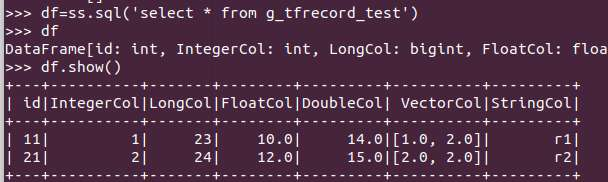
\includegraphics[width=5in,height=1.8in]{table}
\caption{hive table.}
\end{figure}

\textbf{spark写tfrecord,tfrecord其实也是key value的格式,key对应dataframe里的col name. value 自然就是数据本身了。} 
\begin{lstlisting}
df.repartition(10).write.format("tfrecords").option("recordType", "Example").save(path)
\end{lstlisting}

\begin{figure}[H]
\centering
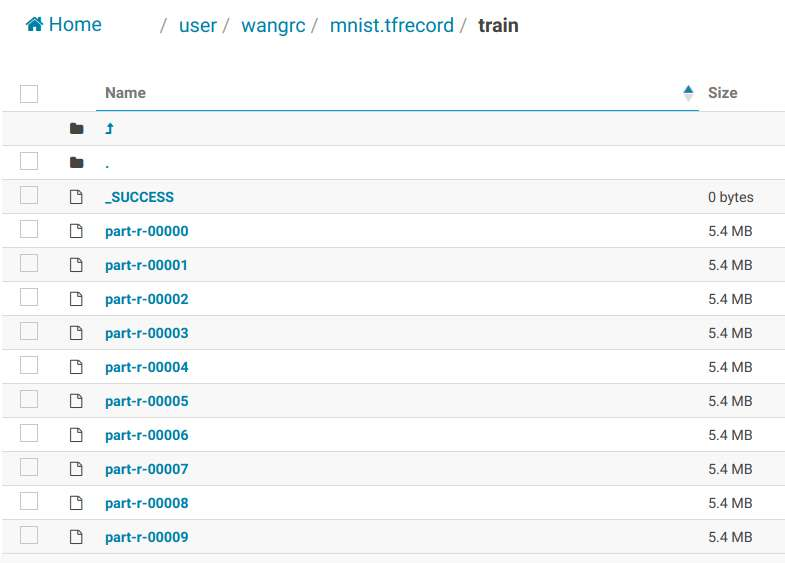
\includegraphics[width=5in,height=3in]{hdfs}
\caption{ hdfs tfrecord}
\end{figure}


\textbf{spark读tfrecord,可以直接读回来成为dataframe}
\begin{lstlisting}
df = spark.read.format("tfrecords").option("recordType", "Example").load(path)
\end{lstlisting}

~\\
注意:使用tensorflow读取hdfs时需要确保CLASSPATH变量设置好,基于安全等一些因素考虑目前没有设置为默认。需要在sh脚本里添加两行 export 代码,加在spark-submit之前就可以了:
\begin{lstlisting}
#!/bin/bash
source /etc/profile
export HADOOP_HOME=/tmp/wangrc/hadoop-2.7.3
export CLASSPATH=$(${HADOOP_HOME}/bin/hadoop classpath --glob)
spark-submit \
--master yarn \
--conf spark.network.timeout=600 \
--conf spark.sql.shuffle.partitions=10 \
--conf spark.executor.memoryOverhead=2048 \
--conf spark.driver.memoryOverhead=2048 \
--executor-cores 1 \
--num-executors 1 \
--executor-memory 4g \
--driver-memory 10g \
train_from_tfrecord.py
\end{lstlisting}

\textbf{tensorflow读tfrecord-推荐使用这种方法,tf dataset 有map方法可以进行decode和一些的特征、数值处理}

\begin{lstlisting}
import tensorflow as tf
tf.enable_eager_execution()
raw_dataset = tf.data.TFRecordDataset(['hdfs://cluster/user/wangrc/test1.tfrecord/part-r-00000'])
for raw_record in raw_dataset.take(2):
    print(repr(raw_record))
\end{lstlisting}

\begin{figure}[h]
\centering
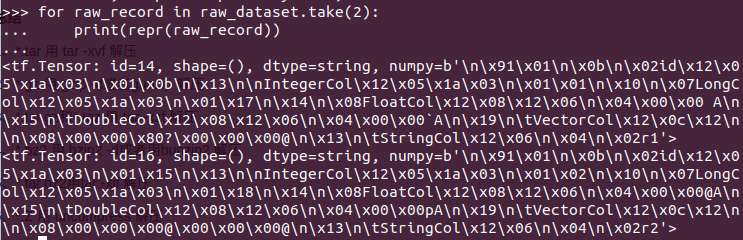
\includegraphics[width=6in,height=1.8in]{print1}
\caption{ 二进制tfrecord}
\end{figure}

\textbf{tensorflow读tfrecord-似乎已经DEPRECATED,方便大家调试的时候用,可以直接看到json格式的key, value。}

\begin{lstlisting}
import tensorflow as tf
record_iterator = tf.python_io.tf_record_iterator(path='hdfs://cluster/user/wangrc/test1.tfrecord/part-r-00000')
for string_record in record_iterator:
    example = tf.train.Example()
    example.ParseFromString(string_record)
    print(example)
\end{lstlisting}

\begin{figure}[H]
\centering
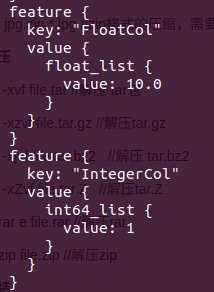
\includegraphics[width=1.5in,height=2in]{print2}
\caption{ json tfrecord}
\end{figure}

\section{模型 Parse \& Train}
建议使用第一种形式读取,tensorflow提供了非常易用的dataset API, 支持源生的tf训练和keras model fit.
\begin{lstlisting}
    feature_description = {
        'label': tf.FixedLenFeature((), tf.int64),
        'features': tf.FixedLenFeature((784), tf.int64),
        }
    def _parse_function(example_proto):
        parsed_feature= tf.parse_single_example(example_proto, feature_description)
        return tf.reshape(tf.cast(parsed_feature['features'], tf.float32),[28,28,1]), \
               tf.cast(parsed_feature['label'], tf.float32)
	dataset = raw_dataset.map(_parse_function,num_parallel_calls=4)
\end{lstlisting}

\begin{figure}[H]
\centering
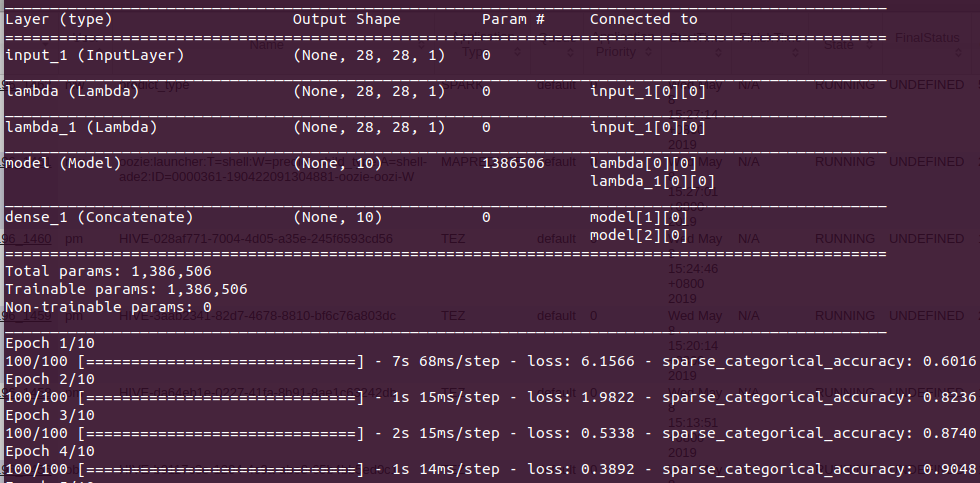
\includegraphics[width=6in,height=4in]{train}
\caption{train}
\end{figure}

\begin{figure}[H] 
\centering
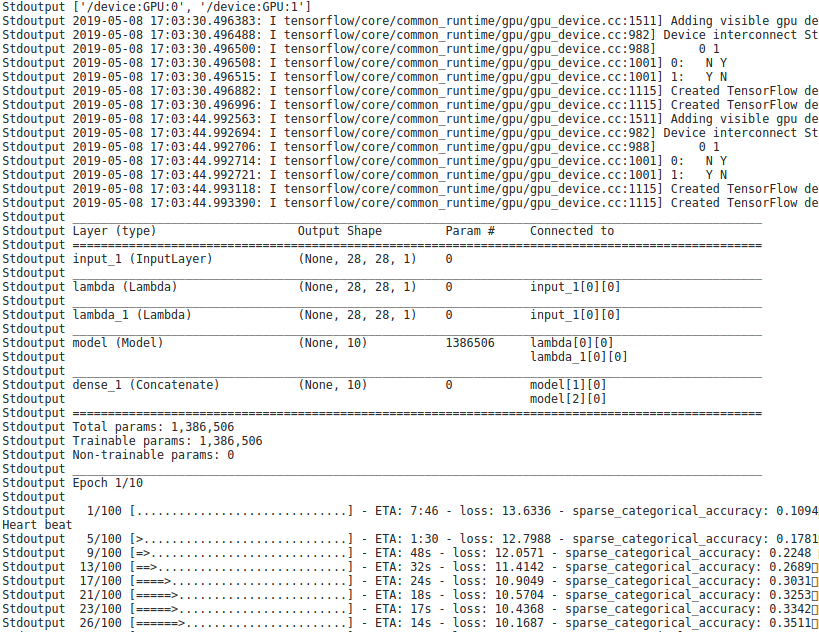
\includegraphics[width=6in,height=4in]{train2}
\caption{train}
\end{figure}

示例代码:
$/user/wangrc/distribute \_ demo$

\section{说好的分布式训练呢?}
我们理想中的分布式训练框架应该有哪些功能呢?
\begin{itemize}
\item 支持spark,hive数据读写
\item 支持任务部署模式,有机制处理挂起或者失败
\item 支持gpu资源弹性分配, 任务级别或者更细节的显卡级别
\end{itemize}
目前有成熟的解决方案吗? Not Found

~\\
\paragraph{GPU训练:}  首先在我们目前的环境中,没有docker, k8s等来做GPU资源管理。在hadoop3.1以后,Databricks、NVIDIA、Google 以及阿里巴巴正在为Apache Spark添加gpu原生支持。相信目前还有很多问题。 目前我们只有spark,hadoop2.7.3,是没有gpu资源管理的。

TensorFlow、PyTorch、XGBoost、LibLinear 这些 AI 引擎的分布式计算能力都有一些问题。TensorFlow 原生支持分布式训练,但不支持容错,一个进程挂了,整个作业就挂了。虽然这还可以通过 checkpointing 解决,但是不容错就不能弹性调度,不能弹性调度就意味着集群利用率可能极差。比如一个有 N 个 GPU 的集群上在运行一个作业,使用了一个 GPU;此时一个新提交的作业要求使用 N 个 GPU,因为空闲 GPU 个数是 N-1,所以这个新的作业不能开始执行,而是得一直等数小时甚至数天,直到前一个作业结束、释放那个被占用的 GPU。这么长时间里,集群利用率< 1/N。关于这个问题的解决方案,百度 PaddleEDL和阿里集团的 XDL做了一些很有益的探索。

实际上,databricks也建议大家尽量在集群中使用单机进行训练。 (我为我自己开脱!)
\begin{figure}[H] 
\centering
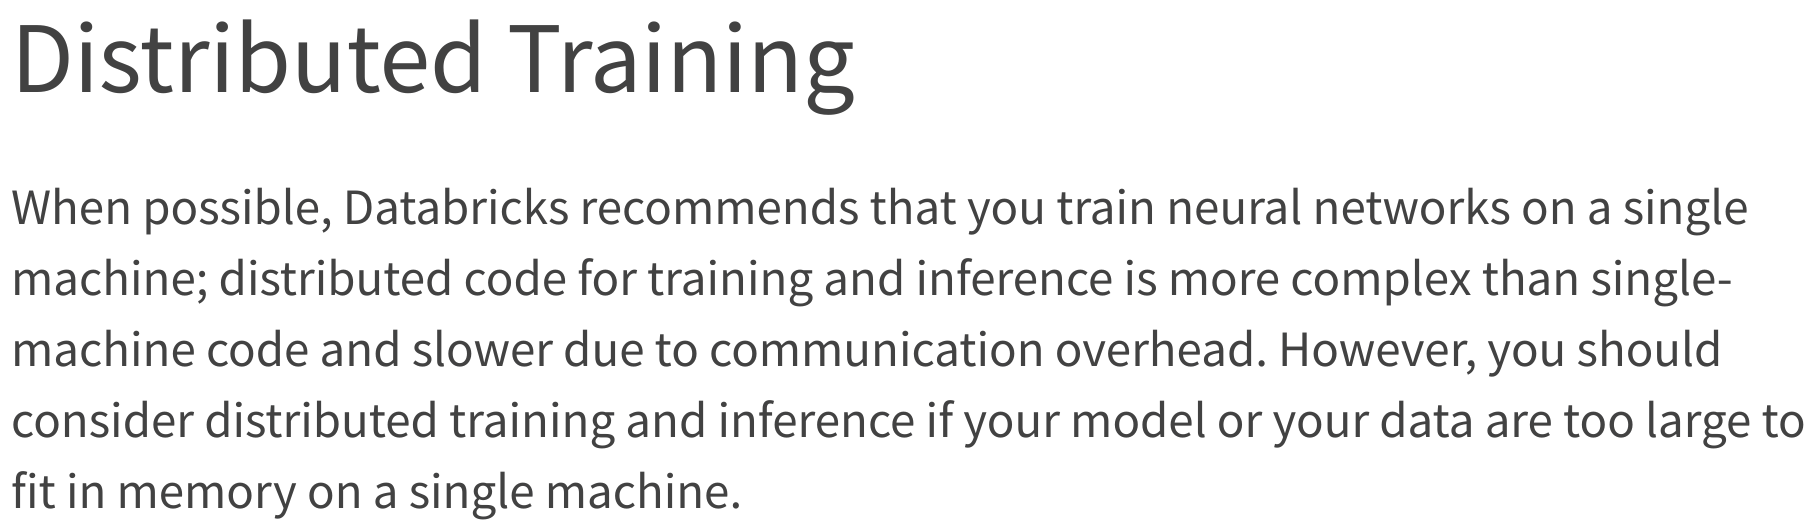
\includegraphics[width=6in,height=1.8in]{dist1}
\caption{Databricks}
\end{figure}

\subsection{Uber的Horovod}

Horovod是uber团队开源一个方便分布式训练的项目。能够非常方便的从单机扩展到多机多卡训练。
\begin{figure}[H] 
\centering
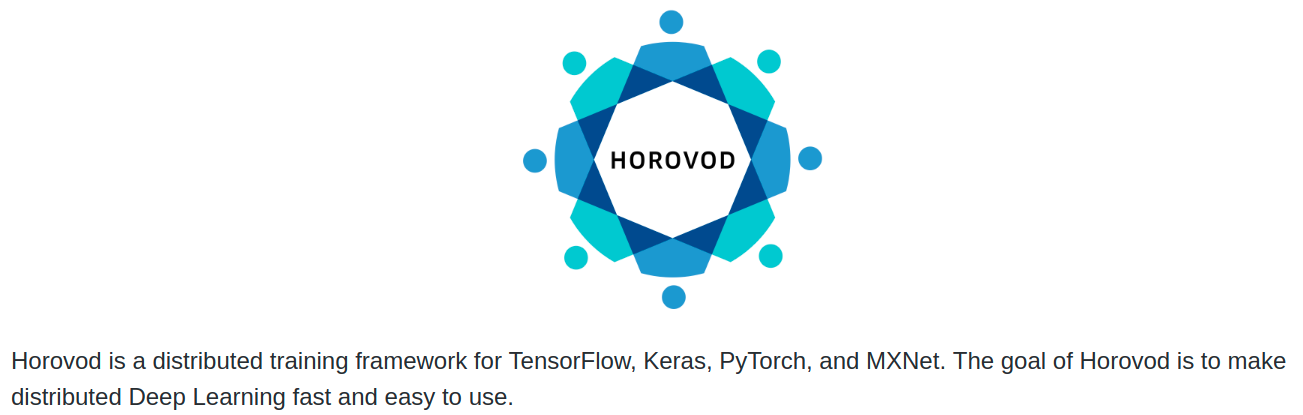
\includegraphics[width=6in,height=1.8in]{hvd}
\caption{hvd}
\end{figure}

\begin{figure}[H] 
\centering
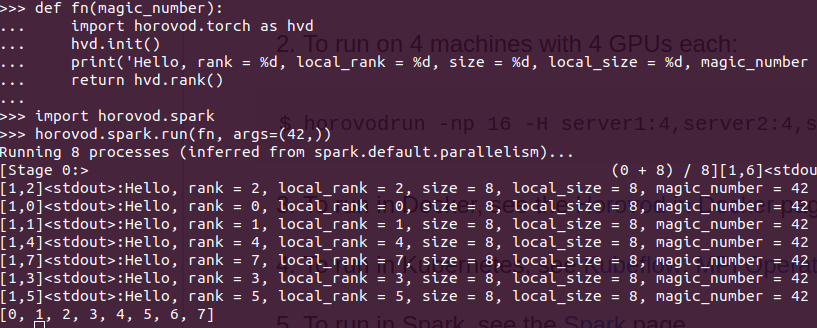
\includegraphics[width=5in,height=1.8in]{hvd_run}
\caption{历尽艰难终于在ha01跑通}
\end{figure}
\textbf{踩过的坑}
~\\

\begin{itemize}
\item 需要openmpi支持,首先openmpi 必须是3.1.2,官方回复:高级版本据说会有卡死问题。

\item tensorflow和hvd必须使用同一版本gcc编译。conda包里的tf与pip hvd不同的gcc不兼容。需要自己重启编译。
 
\item pip包还存在一个已经bug,有些bash命令解析时会多一个括号, 几天前刚刚在github源码中fix。而我非常幸运地刚刚好就遇到了这个bug。。所以需要自己下载源码重启编译,其中遇到的细小问题都记了好几页了。 
 
\item 另外,hvd没有自己的读取hdfs api,需要petastorm的支持。
 
\item hvd号称自己支持tensorflow>=1.12, 然而 1.13就会报 reference error. 直到前天,hvd还在修复一些pytorch nn 的bug 。。
\end{itemize}

不谈hvd api语法等等的学习成本,光是这些千奇百怪的错就已经很折磨人了。

\begin{figure}[H] 
\centering
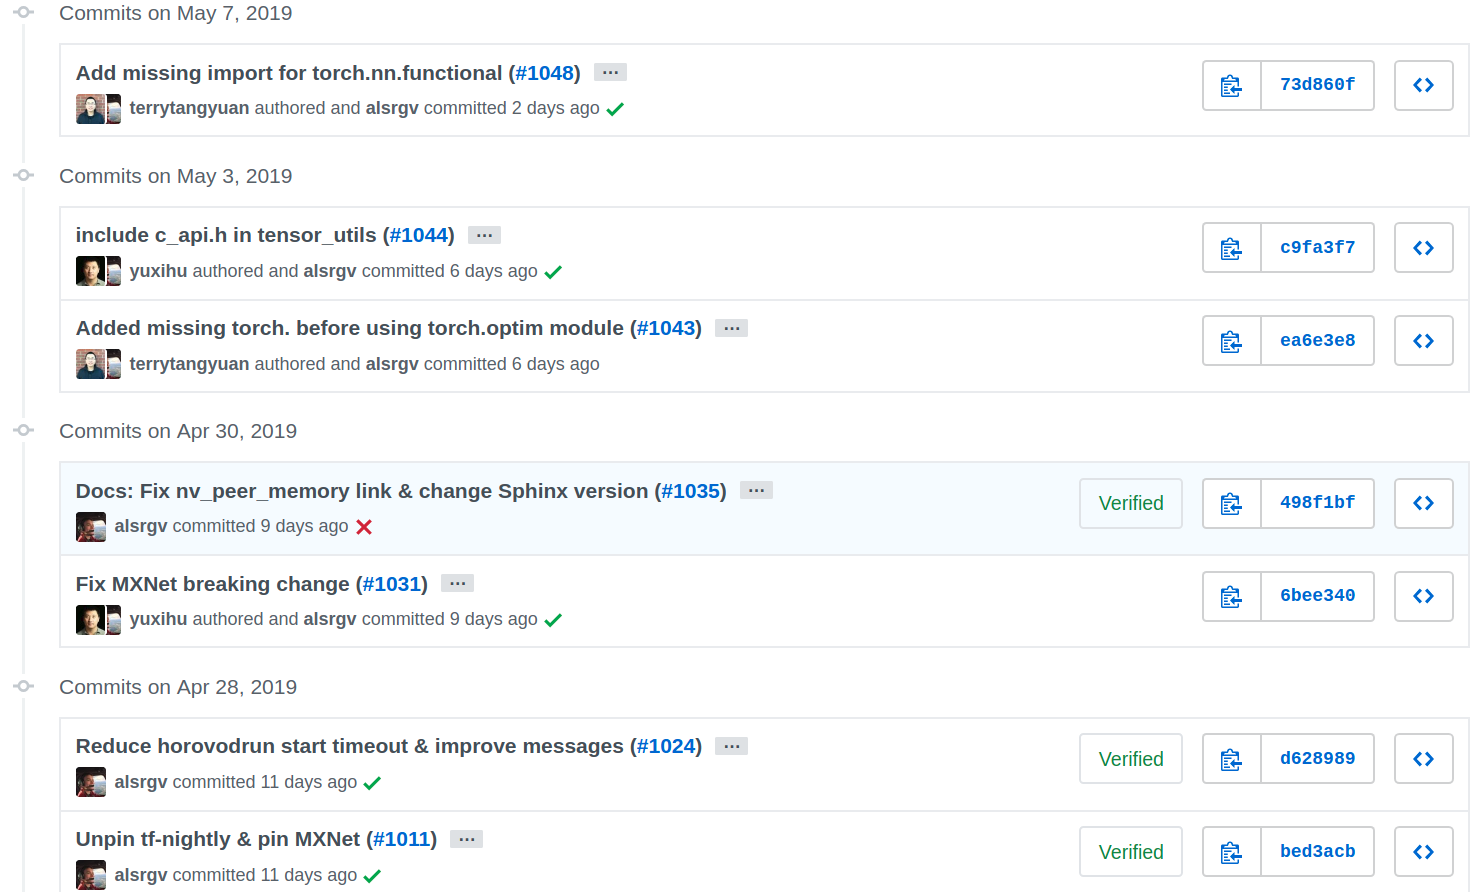
\includegraphics[width=5in,height=1.8in]{hvd_commit}
\caption{hvd commit list}
\end{figure}

再看它的多机多卡需求, 要求所有机器都能互相无密码无权限ssh通,不能有堡垒机的概念了:

\begin{figure}[H] 
\centering
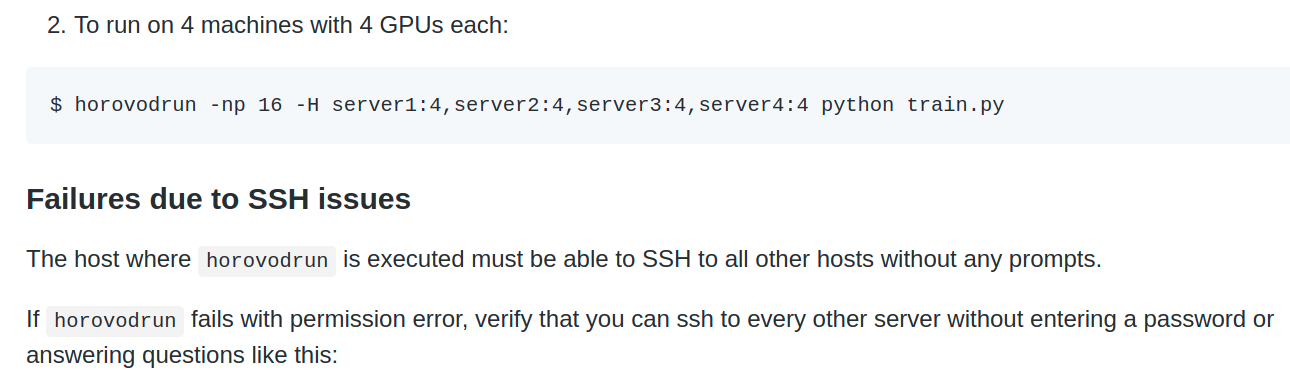
\includegraphics[width=6in,height=1.8in]{hvd_ssh}
\caption{what??}
\end{figure}

这和我一台一台机器ssh上去手动跑命令有什么区别???

\subsection{多机多卡训练}
其实,在推荐系统领域,并没有很庞大的深度学习网络。不像CNN或者RNN 一个kernel就有很多参数。一块GPU 训练FFM跑10亿的数据,也就15分钟以内就跑完一轮了。

~\\
如果大家真的有需求,需要训练一个超大的深度学习网络,大到2块GPU不能满足你训练要求。 推荐使用原生的tensorflow 分布式训练方法: 在测试环境里写好master,worker节点和端口,到每台机器上去手动运行,先训练好你的模型。保存好模型到线上hdfs, 线上单节点预测。在测试环境里随便折腾,5台机器7块GPU都可以一起训练。

\paragraph{Q: } 我不死心,我就要用多块GPU。 我可以写一个sh脚本,在一个机器上操作吗? 我可以建立定时任务大家一起跑分布式吗?
\paragraph{A: } 建议不要。 写sh脚本基本不可能。涉及到权限问题,线上不可能让一个sh脚本操作整个集群的。 定时任务也不好,最主要的还是没有资源管理,如何知道你的任务成功与否?跑死机了谁来解决 ?
\end{CJK*}
\end{document}

























